\chapter{The Robot Models}

\section{Soccerbot}

\begin{figure}[htp]
  \centering
  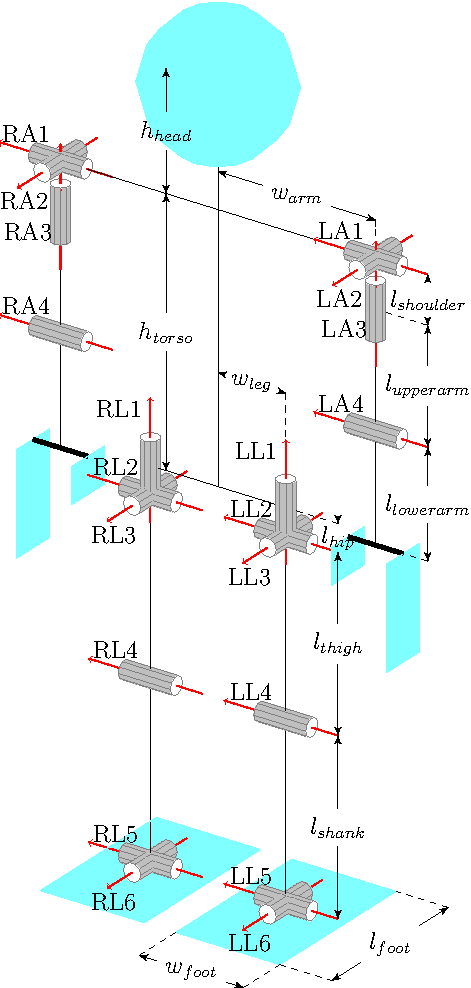
\includegraphics[height=0.7\textwidth]{fig/soccerbot056}
  \caption{Overview of the degrees of freedom of the Soccerbot}
  \label{fig:soccerbotdof}
\end{figure}

\begin{table}
\label {table:perceptorNames}
\caption{Perceptor and effector names}
\begin{center}
\begin{tabular}{|l|l|l|l|}
\hline
{\bf Connection between}  & {\bf Joint type} & {\bf Perceptor name}& {\bf
Effector name} \\
\hline
%Klaus: how do I get underscore character?
Shoulder - body  & Universal joint & laj1\_2  raj1\_2 & lae1\_2   rae1\_2 \\
\hline
Upper arm - shoulder  & Hinge joint & laj3  raj3 & lae3   rae3 \\
\hline
Forearm - upper arm  & Hinge joint & laj4  raj4 & lae4   rae4 \\
\hline
Hip - body  & Hinge joint & llj1  rlj1 & lle1   rle1 \\
\hline
Upper leg - hip & Universal joint & llj2\_3  rlj2\_3 & lle2\_3   rle2\_3 \\
\hline
Lower leg - upper leg & Hinge joint & llj4  rlj4 & lle4   rle4 \\
\hline
foot - lower leg & Universal joint & llj5\_6  rlj5\_6 & lle5\_6   rle5\_6 \\
\hline
\end{tabular}
\end{center}
\end{table}


%Later: HOAP-2, NEC Papero (I already did a model in Blender), CITIZEN Eco-Be!, VisiON 4g (Fabio Dalla Libera is working on that), AIBO via RoSIML importer

%%% Local Variables: 
%%% mode: latex
%%% TeX-master: "user-manual"
%%% End: 
